%
% Author kit for UCSC graduate classes in computer systems.
%
% Author guidelines and sample document in LaTeX 2e.
%

\documentclass[10pt,twocolumn]{article}

% Use the USENIX style file
\usepackage{usenix}

% Here are a bunch of useful packages
\usepackage{cite}
%\usepackage[]{biblatex}
\usepackage{xspace,verbatim}
\usepackage{subfig}
\usepackage{graphicx}
\usepackage{epstopdf}
\usepackage{float}
\usepackage{listings}
\usepackage[hyphens]{url}

% subfig default captions are too small.  This fixes it.
\captionsetup[subfloat]{font=normalsize}

% Redefine the percentage of the page that can be used for floats (figures,
% tables, etc.)
\renewcommand\floatpagefraction{.9}
\renewcommand\dblfloatpagefraction{.9}
\renewcommand\topfraction{.9}
\renewcommand\dbltopfraction{.9}
\renewcommand\bottomfraction{.9}
\renewcommand\textfraction{.1}
\setcounter{totalnumber}{10}
\setcounter{topnumber}{10}
\setcounter{dbltopnumber}{10}
\setcounter{bottomnumber}{10}

% Don't allow widows or clubs - single lines at the start/end of a column
\widowpenalty=10000
\clubpenalty=10000

\newcommand{\latex}{\LaTeX\xspace}
\newcommand{\unix}{\textsc{Unix}\xspace}

\pagestyle{plain}

%------------------------------------------------------------------------- 
\begin{document}

\title{A Music Recommender System Based on Emotion}

\author{
{\rm Patrick Cudahy} \\
\textit{pcudahy@ucsc.edu}
\and
{\rm James Byron} \\
\textit{jbyron@ucsc.edu}
\and
{\rm Brady Goldman} \\
\textit{btgoldma@ucsc.edu}
}

\maketitle

\begin{abstract}
The rise of the internet has accompanied an increasing demand for entertainment on demand, including digital music.  To satisfy the demand for instant access to music, online music streaming services offer huge song libraries for listeners to enjoy.  The rising popularity of online music streaming services has also led to competition between different streaming services to keep listeners' attention, and to accomplish this, streaming services use recommender systems to automatically generate personalized playlists for each music listener.  Currently recommender systems utilize each user's listening history or the listening habits of similar users to generate lists of novel music to play.  Users may, however, wish to listen to music that expresses a particular emotional motif, and current recommender systems may not effectively serve this purpose.  We propose a recommender system that generates recommendations for music based on the emotions that a listener selects.  We use word2vec to generate lists of words that are typically associated with different emotions.  We use the list of emotionally correlated words to discover songs that have a high degree of cosine similarity with them using doc2vec.  We describe our model and evaluate its performance using crowd-sourced classification of the emotions expressed in song lyrics.
\end{abstract}

\section{Introduction}
Music can make an emotional connection with listeners.  Music typifies graduation ceremonies, weddings, funerals, religious ceremonies, and political inaugurations with the fanfare and consequence that they typify.  In more casual settings, music sets the mood in restaurants and grocery stores, provides emotional signaling in motion pictures and commercials, and accompanies drivers during long voyages to ward off boredom.  Music carries emotional signals in its tones and lyrics that listeners enjoy and resonate with.

The availability of digital music through the internet has enabled fans to discover and enjoy both familiar and novel types of music.  While services like iTunes \cite{a16} allow customers to purchase their music online, other business models for delivering music to listeners have allowed customers to enjoy their favorite songs and easily discover new songs and artists.

Digital music streaming services like Pandora \cite{a12} and Spotify \cite{a13} offer a virtually unlimited library of music to subscribers who pay for the service either through a monthly fee or advertisements.  Subscribers enjoy the option to listen to any music genre without having to buy each song or album, and the large music library ensures that listeners can find music for any occasion.  The streaming services profit from listeners who remain paying subscribers or who continue to listen to advertisements and therefore each service seeks to capture and retain every music listener's attention.  With the goal of improving listener experience increasing subscriber retention, music streaming services automatically create playlists to make continuous listening convenient, effortless, and suitable for each user's listening preferences.

Music streaming services like Pandora and Spotify construct playlists of recommended music based on each user's listening preferences.  The music recommender system within each streaming service offers music that is typically similar to the songs and artists that each user has played before.  The streaming service may analyze a user's listening history to identify similar songs when dynamically constructing a user-specific playlist.  Alternatively, each user's listening history may be compared with other users to suggest songs for the playlist that similar users have enjoyed.  Both strategies for recommending music rely on the preferences of listeners as conveyed through their listening patterns and history.  Current recommender systems offer the benefit of presenting diverse music to each listener, but user historical and pattern-based recommender systems do not include the emotional state of the listener as a selection criterion.

Musical interests are personal and also subject to change with different moods and over time.  Therefore, music recommender systems based purely on user history do not suit every important use case for music recommender systems.  We propose a solution to this problem with a music recommender that creates dynamic playlists based on the mood of the lyrics to music.  Our recommender system identifies songs with the most similarity to the user's current mood.  We have identified several core emotions that typify the feelings expressed in many popular songs, and we extract emotional keywords from a corpus of song lyrics that correspond to each emotion.  To initially determine a listener's mood, our model may utilize either a user-provided emotional keyword or the emotion keyword that corresponds to a song that the user has selected to play.

In the following sections we discuss related work and background to our approach, the database of song lyrics that we use, our model implementation, and our experimental results.

\section{Data Description}
To design and evaluate our model, we used a publically available list of lyrics available from Kaggle. \cite{a14}  The list was generated by crawling the MetroLyrics catalog of music lyrics. \cite{a15}  The dataset includes lyrics for approximately 380,000 popular songs in English.  The dataset includes fields for song title, release year, artist, genre, and lyrics. We prepared our dataset by filtering stop words and removing instrumental songs that have no lyrics.  We also exclude songs that have lyrics of fewer than 20 words since our model relies on word vectors that are at least 20 words long.

\section{Related Work}
\subsection{Emotion in Music Recommender Systems}
Music recommender systems are a challenging area of research.  Especially challenging are the goals of recommending music to new users to a music streaming service, predicting which users will enjoy a new song or album when it is added to the streaming library, and the evaluation of the music recommender system. \cite{a1}  Music recommender systems are different than film recommenders in several ways.  Songs are typically shorter than a film, and a listener will often listen to many songs consecutively but only one film at a time.  Also, songs have a high emotionality compared with films in general.  Finally, users are sometimes willing to accept repeated recommendations to songs, but they are less likely to enjoy watching the same film repeatedly.  Music recommenders must respond to users' sporadic inputs of expressing like and dislike for music by playing or skipping songs, and the music recommender must constantly present music that is both novel and sufficiently diverse to attract the listener's continued attention.  User mood, location, and activity often affect the listener's perception of appropriateness for a particular song, and the quality of a music recommender should reflect its ability to respond to the user implicitly.

Recent work has explored techniques to include musical emotion as a factor in recommender systems.  Musical key, tempo, and melody characterize emotional features of music.  Film music, which closely follows the dialogue in the film, reflects the emotion of the scene.  Previous work has demonstrated a technique to learn the musical features that reflect the emotions communicated in film text and apply those features to other music. \cite{a2}  Other research used machine learning to discover correlations between musical lyrics and emotions. \cite{a3}  A psychological linguistic dictionary assisted the machine learning algorithm in discovering the emotional connotation of English words.  This approach differs from others in that it extracts emotions from text using an expert-defined psychological linguistic model rather than syntactical text analysis.

\subsection{Word2Vec and Doc2vec}
The Word2vec algorithm discovers semantic analysis tool for discovering relationships between words.  It converts words and word contexts into vectors \cite{a4,a5,a6}, and the vectors resemble a shallow neural network, the smaller number of features compared with a neural network allows Word2vec to require less memory and computational power than a neural network.  To create the context for each word, Word2vec uses either a continuous bag-of-words (CBOW) or skip-gram model.  The CBOW model is suitable for predicting a central word based on its context of words, and the skip-gram is optimal for predicting a context of words based on a central word.   Word vector representations can also be added or subtracted together to combine different concepts.  For example, the vector representations for king, man, and queen hold that king - man = queen.

Doc2vec is an extension of Word2vec to utilize an entire paragraph or document as the context window for each word. \cite{a7,a8}  Doc2vec predicts words in a document context based on a word.  Doc2vec has a lower error rate than Word2vec does in some cases.

\subsection{Other Approaches}
Word2vec is a distributional approach to word representations using the values in the vectors that correspond to the distribution of the probability that two words appear in the same context.  An alternative to the distributional approach is the counting approach, which creates a sparse matrix showing how many times each word appears in the context of every other word in the corpus.  The counting approach requires more memory than the distributional approach because it uses a large sparse matrix.  Initial results with Word2vec and Doc2vec showed that their performance was better than the older counting approaches like Latent Semantic Analysis (LSA), but recent work indicates that LSA may be more effective than Word2vec on small corpora. \cite{a10}  Small corpora also require smaller co-occurrence matrices, which makes LSA still more attractive in such scenarios.  Other work suggests that parameter tuning can reduce or eliminate any performance differences between different analysis techniques. \cite{a11}
  
\section{Implementation}


\begin{table}[!hb]
\begin{center}
 \begin{tabular}{ | c | c | } 
 \hline
\textbf{Emotion} & \textbf{Associated Works} \\ [0.5ex] 
 \hline
Love & Love, Lust \\ 
 \hline
Hate & Hate, Anger \\ 
 \hline
Happy & Happy \\ 
 \hline
Sad & Sad \\ 
 \hline
\end{tabular}
\caption{Each emotion correlates with a list of words in the corpus of song lyrics.}
\end{center}
\end{table}

\subsection{Preprocessing}

Song lyric records from the MetroLyrics dataset were first filtered to remove songs with an empty genre attribute or genres labeled "Not Available" or "Other" as well as an empty lyrics section.  Each set of song lyrics were then tokenized by word using the TweetTokenizer model from NLTK.  We chose this tokenizer over NLTK's default tokenizer because it does not split contractions.  We then used stratified sampling to sample 2000 song lyrics from each genre, bringing the total sample size to 20000 lyrics.  

\subsection{Doc2Vec Generation}

We first selected seed words for each of the emotional categories we chose for use in generating a list of 50 most similar wordsfor each category (Table 1).  We chose these emotional categories because each one has a distinct, respective opposite that we can use as negative examples.  The seed words were chosen based on minimizing the appearance of noise within the generated similar word list.

To generate the word lists, we used a pre-trained Word2Vec model taken from the Google News dataset, which contains a 300-dimensional vector representation of 3 million different words and phrases \cite{a6}.  For each emotional category, we generated a list of 50 most similar words based on cosine similarity using the seed words of the emotional category as positive examples and the seed words of its opposite emotional category as negative examples.  We used Gensim's \texttt{most\_similar()} function to perform this task.  We subsequently used the word vectors of the similar words to create corresponding Doc2Vecs for each emotional category.

Because we do not care about the position of each word relative to one another in the collection of related words to an emotion category, we simply take the bag-of-words approach to our Doc2Vec design by creating an averaged vector for all word2vec occurrences in the document.  We use this approach both for creating vectors for the emotion categories and each song lyric.

\subsection{Measurement}

After normalizing the vectors for emotional categories and song lyrics, we measured similarity between each song lyric document vector and emotional category vector by use of cosine similarity.

\section{Experimental Results}
Testing and evaluating our music recommender system was a two-step process. First, the accuracy of the model's song classification was evaluated using human surveys on a small set of test songs. We then ran the algorithm on the entire corpus of song lyrics and displayed the results with histograms to see what insights they might provide on the emotional tendencies of different music genres.

\subsection{Song Emotion Evaluation}
\begin{figure}[!htb]
\centering
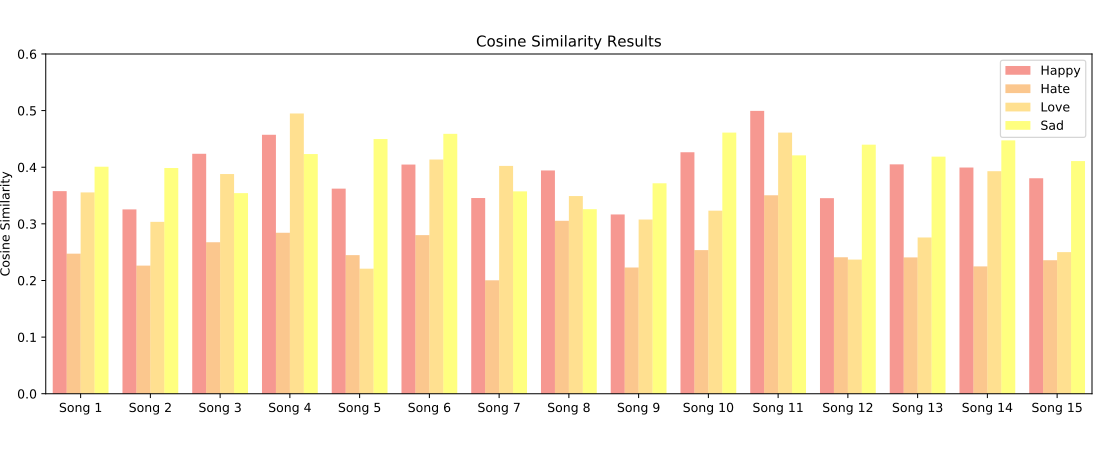
\includegraphics[width=\textwidth]{test_cos.png}
\caption{Figure 1(a): Song cosine similarity to emotion class}
\label{fig:digraph}
\end{figure}
\begin{figure}[!htb]
\centering
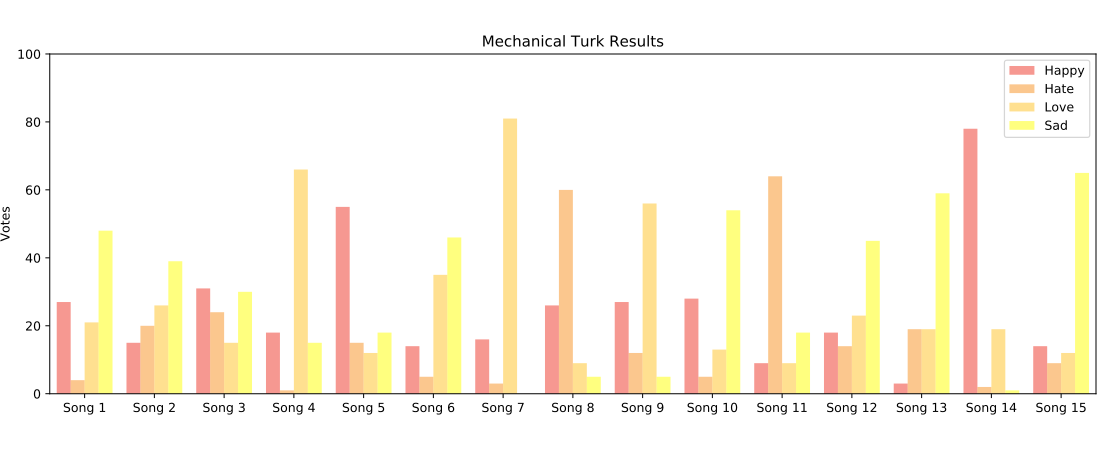
\includegraphics[width=\textwidth]{test_vote.png}
\caption{Figure 1(b): Song emotion classified by Amazon Mechanical Turk survey}
\label{fig:digraph}
\end{figure}
We used Amazon Mechanical Turk to evaluate our music recommender model's ability to classify the primary emotion conveyed by a song. Using a set of fifteen example songs from across multiple genres, our music recommender algorithm calculated the cosine similarity of each song to the four emotion categories. At the same time, a group of one hundred Turkers reviewed the lyrics of each song without the song title or artist.  The Amazon Turk reviewers selected which of the four emotion classes each song most closely resembled. The results of both tests are shown in figures 1 and 2, respectively. The algorithm achieved an accuracy of .66, ranking the same emotion class identified by the Turkers as having the greatest cosine similarity to the test song in ten out of fifteen instances.  We believe that further work to identify a more specific corpus of words for each emotion may improve the accuracy of our model.  We leave this task to our plans for future work.

\subsection{Genre Classification}
\begin{figure}[!htb]
\centering
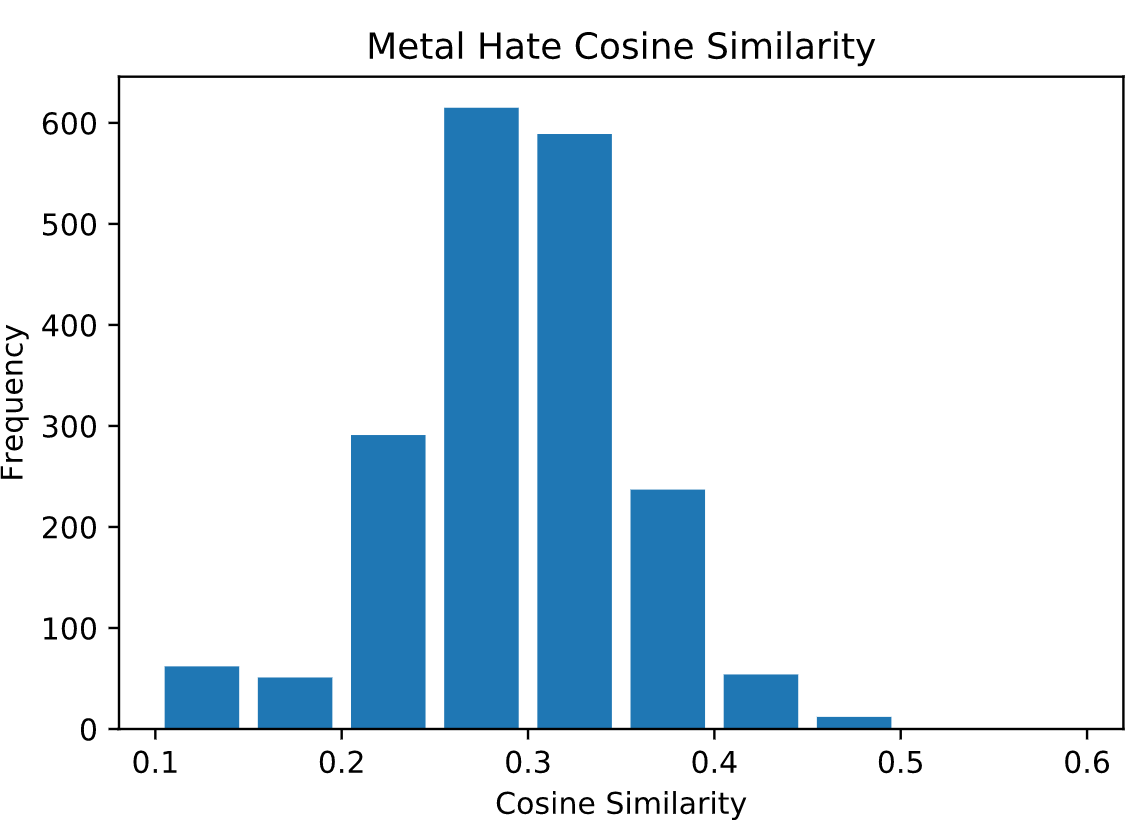
\includegraphics[width=3.125in]{metal_hate.png}
\caption{Figer 2(a): Distribution of cosine similarites to "Hate" emotion class for the Metal genre}
\label{fig:digraph}
\end{figure}
\begin{figure}[!htb]
\centering
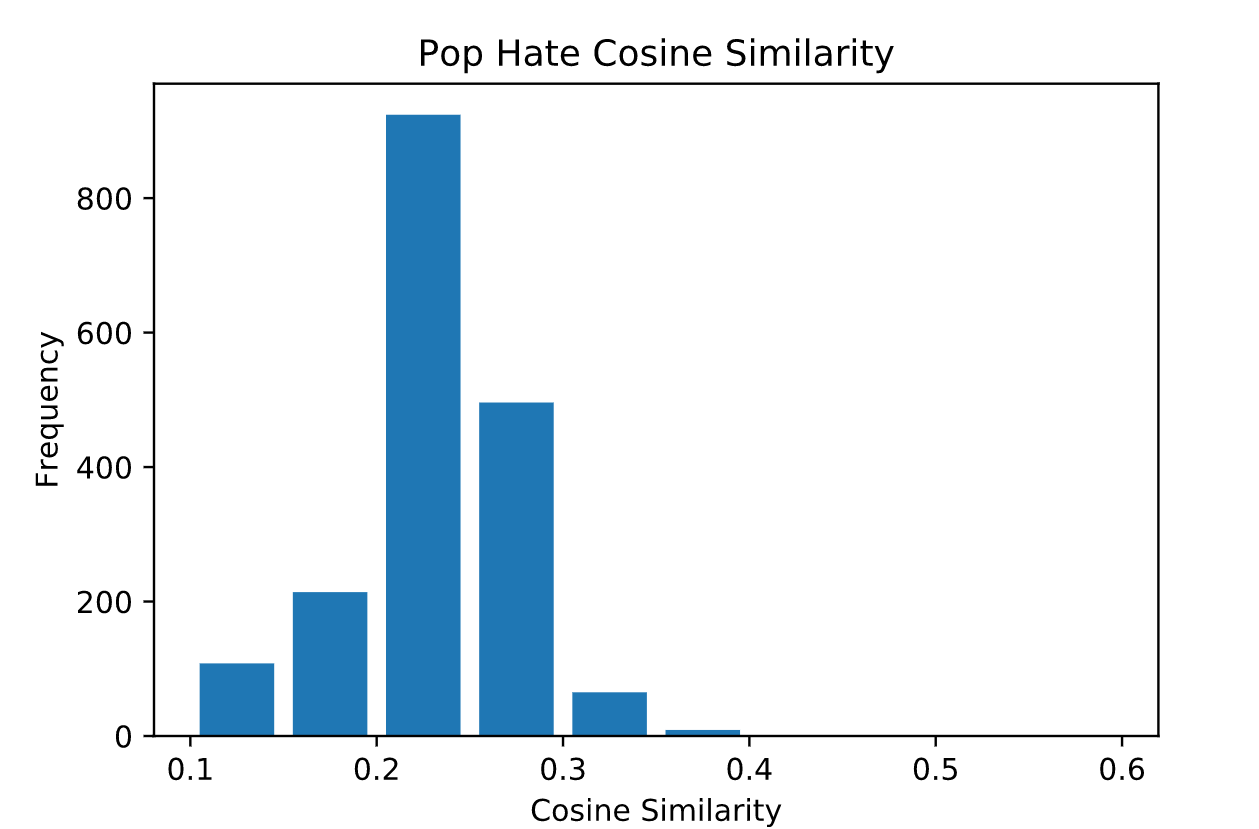
\includegraphics[width=3.125in]{pop_hate.png}
\caption{Figure 2(b): Distribution of cosine similarites to "Hate" emotion class for the Pop genre}
\label{fig:digraph}
\end{figure}
Using the song lyric corpus obtained from Kaggle \cite{a14}, we selected the emotion of two thousand songs from each of ten musical genres. We ran the songs through our algorithm to calculate their cosine similarity to each list of emotional words. Using these cosine similarities, we created four histograms for each genre, showing the distribution of similarities across each of the four types of emotion. Above all, the graphs show that songs within any given genre vary widely in regards to which emotion they portray. For some genres, the cosine similarities of songs to emotions are evenly distributed across all four types of emotion.  For other genres, different songs have widely different cosine similarities for a given type of emotion.

Some of the histograms give insight into overall trends within a genre. One such trend can be seen in figures 3 and 4. The histograms clearly show that the Metal genre trends towards the hate/anger emotion, while at the same time, Pop songs tend to have a low cosine similarity to the hate/anger emotion. While emotional trends within broadly defined genres are limited due to the wide variety of songs within such genres, the set of histograms produced by our music recommender system provides insight into how various genres relate to different emotions.  A genre's songs may therefore be either split, evenly spread, similar, or dissimilar to particular emotions. The full set of forty histograms, ten genres each with four emotion classes, can be accessed on our project's github page at \url{https://github.com/BGoldman1989/song-recommender/}.

\section{Conclusion and Future Work}
Music recommender systems make listening to streaming music easier by automatically generating playlist for listeners based on their own listening history or the histories of other listeners.  While many music recommenders use historical listening patterns to generate playlists, we have proposed a music recommender system that uses emotional keywords to discover correlation between songs to generate playlists.  We expect that emotional playlists will improve the listener experience by including songs that feature emotions similar to what the listener wants to hear at any given moment.  Our algorithm generated lists of words that are closely associated with each emotional keyword, but we discovered that the lists of emotional words included songs that were both positively and negatively associated with each income.

In future work, we plan to further refine our algorithm by implementing techniques for excluding songs that exhibit an emotion that is the opposite of what the user wants to hear.  We plan to explore the benefit of using latent semantic analysis to discover correlations between lists of emotional works and individual songs.  We also hope to write and submit a conference paper detailing our algorithm and our experimental results.


\bibliographystyle{abbrv}
\bibliography{references}

\end{document}\grid
